\subsubsection{UCE1.1 - Visualizzazione errore campo nome}
\begin{figure}[H]
    \centering
    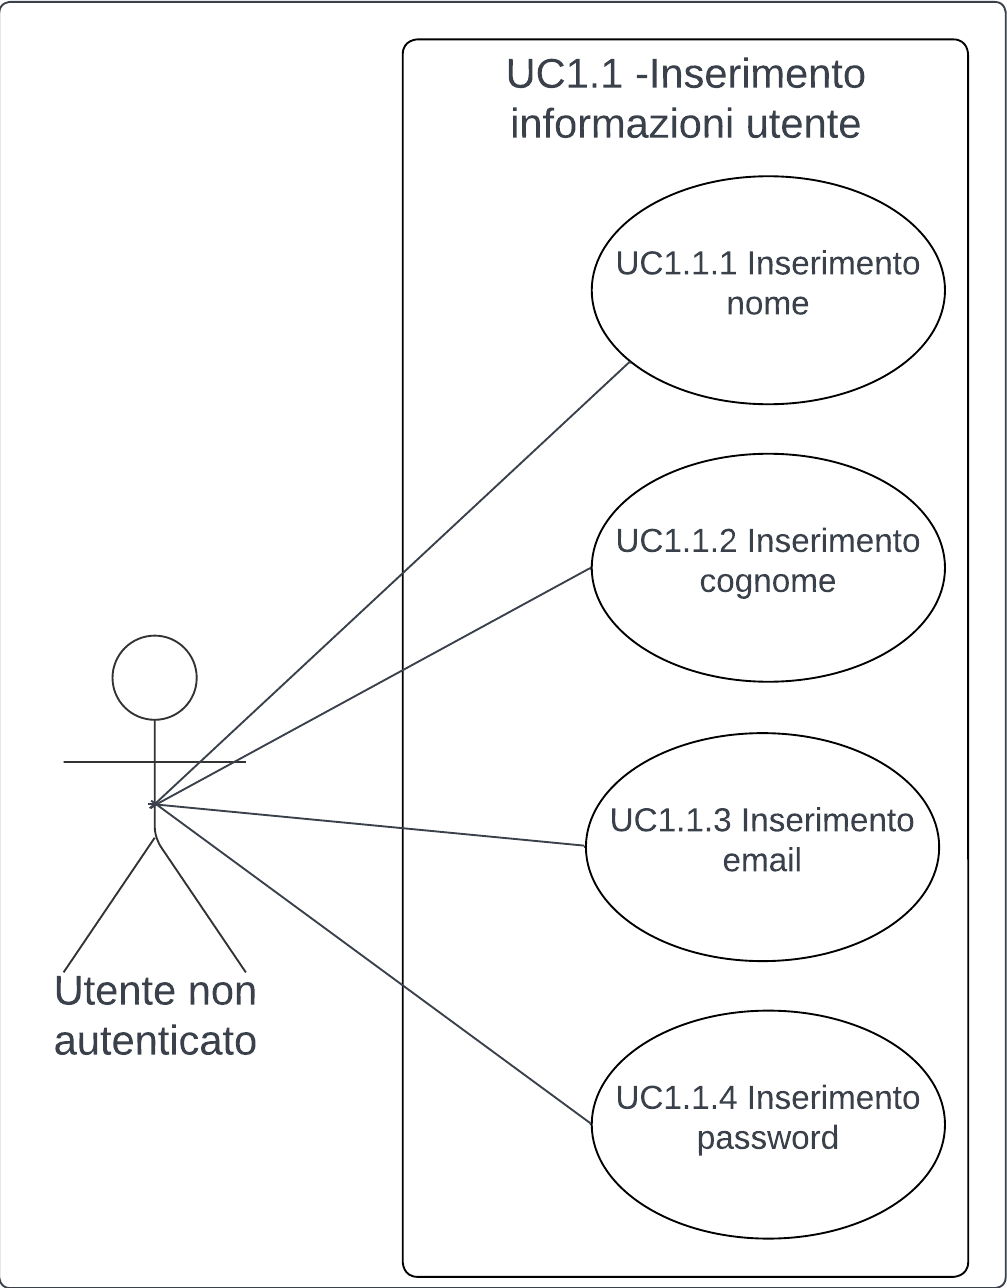
\includegraphics[width=0.75\linewidth]{ucd/UCD1.1.png}
\end{figure}
\textbf{Attori}:
\begin{itemize}
    \item $\textit{Attore}_G$ non autenticato.
\end{itemize}
\textbf{Precondizioni}:
\begin{itemize}
    \item L'utente ha inserito un nome non valido.
\end{itemize}
\textbf{Postcondizioni}:
\begin{itemize}
    \item L'utente visualizza un messaggio di errore e $\textit{sistema}_G$ corregge l'errore.
\end{itemize}
\textbf{Scenario principale}:
\begin{enumerate}
    \item L'utente visualizza un errore;
    \item L'utente modifica il campo sbagliato.
\end{enumerate}
\textbf{Scenario alternativi}:
\begin{enumerate}
    \item L'utente sceglie di annullare la procedura di inserimento dati.
\end{enumerate}